\documentclass{standalone}
\usepackage{tikz}
\usetikzlibrary{angles,quotes}

\begin{document}
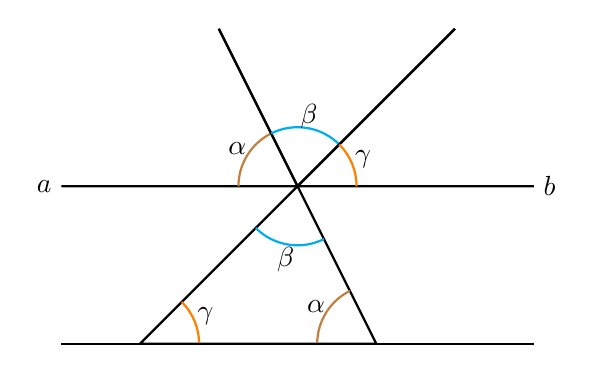
\begin{tikzpicture}
  \coordinate (x) at (3,0);
  \coordinate (y) at (0,0);
  \coordinate (z) at (2,2);
  \coordinate (p) at (1,4);
  \coordinate (q) at (4,4);

  \node[left] (a) at (-1,2) {\(a\)};
  \node[right] (b) at (5,2) {\(b\)};
  \coordinate (c) at (-1,0);
  \coordinate (d) at (5,0);

  % main triangle
  \draw[thick]
  (x) pic["$\alpha$", draw=brown, -, angle eccentricity=1.2, angle radius=0.75cm]
  {angle=z--x--y}
  -- (y) pic["$\beta$", draw=cyan, -, angle eccentricity=1.25, angle radius=0.75cm]
  {angle=y--z--x}
  -- (z) pic["$\gamma$", draw=orange, -, angle eccentricity=1.2, angle radius=0.75cm]
  {angle=x--y--z}
  -- cycle;

  % angles above parallel line
  \draw[thick] (a) -- (z) -- (p)
  pic["$\alpha$", draw=brown, -, angle eccentricity=1.2, angle radius=0.75cm]
  {angle=p--z--a};
  \draw[thick] (p) -- (z) -- (q)
  pic["$\beta$", draw=cyan, -, angle eccentricity=1.2, angle radius=0.75cm]
  {angle=q--z--p};
  \draw[thick] (q) -- (z) -- (b)
  pic["$\gamma$", draw=orange, -, angle eccentricity=1.2, angle radius=0.75cm]
  {angle=b--z--q};

  % extend the base of the triangle
  \draw[thick] (c) -- (d);
\end{tikzpicture}
\end{document}
